\documentclass[11pt]{article}
\usepackage{geometry}                % See geometry.pdf to learn the layout options. There are lots.
\geometry{letterpaper}                   % ... or a4paper or a5paper or ... 
%\geometry{landscape}                % Activate for for rotated page geometry
%\usepackage[parfill]{parskip}    % Activate to begin paragraphs with an empty line rather than an indent
\usepackage{graphicx}
\usepackage{amssymb}
\usepackage{amsmath}
\usepackage{epstopdf}
\usepackage{hyperref}
\usepackage{natbib}
\DeclareGraphicsRule{.tif}{png}{.png}{`convert #1 `dirname #1`/`basename #1 .tif`.png}


\graphicspath{
{/Users/Andy/Cruises_Research/Chipod/EQ08/}
{/Users/Andy/Cruises_Research/Chipod/EQ08/Figures/}
}

\title{EQ08 Chameleon-$\chi$pod Comparison Notes}
\author{Andy Pickering}
%\date{}                                           % Activate to display a given date or no date


\begin{document}
\maketitle

\tableofcontents
\newpage

%~~~~~~~~~~~~~~~~~~~~~~~~~~~~~
\section{About}

This document contains notes related to tests of the $\chi$pod method using EQ08 Chameleon data. This is similar to an analysis done with EQ14 data. The plan was to:

\begin{enumerate}
\item Process raw Chameleon profiles and apply calibrations.
\item Apply $\chi$pod method to Chameleon FP07 T` signal, and estimate $\chi$ and $\epsilon$.
\item Compare these values to the `true' values: the processed Chameleon data using shear probe data.
\item Examine the sensitivity of the $\chi$pod results and comparisons to variable parameters in the $\chi$pod calculation.
\end{enumerate}



%~~~~~~~~~~~~~~~~~~~~~~~~~~~~~
\section{Data and Methods}

The raw Chameleon profiles are read and calibrated with \verb+run_eq08_AP.m+, which I modified from the original \verb+run_eq08.m+. This script calls:
\begin{itemize}
\item \verb+tag_file_eq08.m+
\item \verb+raw_load.m+
\item \verb+cali_eq08.m+
\end{itemize}

The $\chi$pod method is applied to each profile in \verb+Calc_Chi_eq08_AP.m+, using the same methods used on CTD-$\chi$pod data. The core calculations are done in \verb+get_chipod_chi.m+; much of the other functions are to organize and prepare the data for this calculation.



\clearpage
\newpage
%~~~~~~~~~~~~~~~~~~~~~~~~~~~~~
\section{Summary of Data}

Figure \ref{cham_sum} shows a summary of the processed Chameleon data from the file \verb+eq08_sum.mat+. Figure \ref{chi_sum} shows the corresponding summary for the $\chi$pod method applied to the data. Qualitatively, the timing, depth-structure, and magnitudes seems to agree well. Differences will be examined more quantitatively later in this document.

\begin{figure}[htbp]
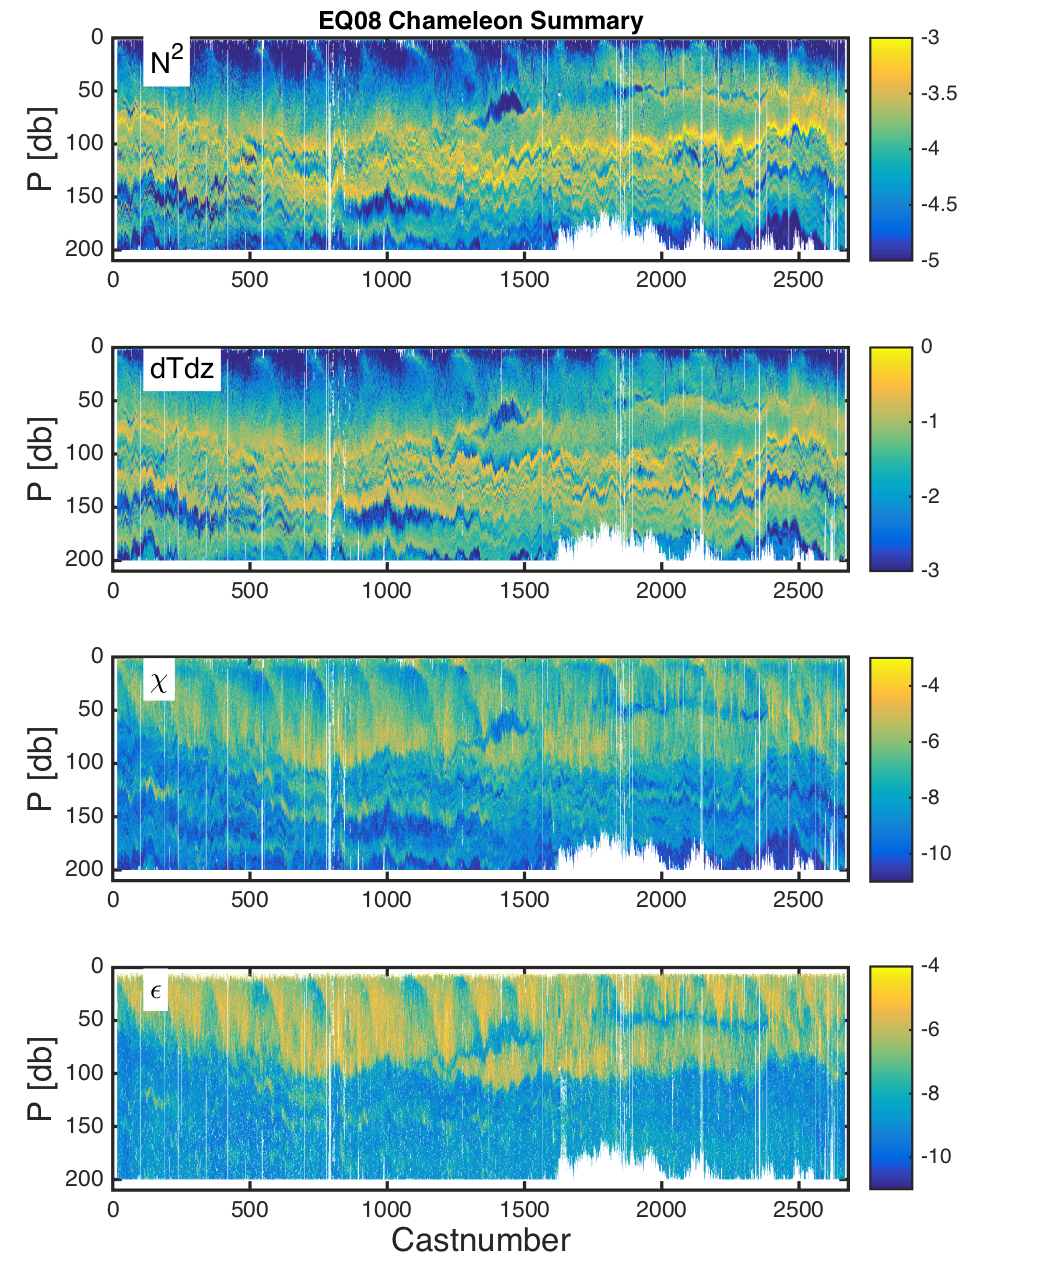
\includegraphics[scale=0.95]{EQ08_PreProc_Summary.png}
\caption{Summary of processed Chameleon data from EQ08 (already processed, NOT what I processed).}
\label{cham_sum}
\end{figure}

\begin{figure}[htbp]
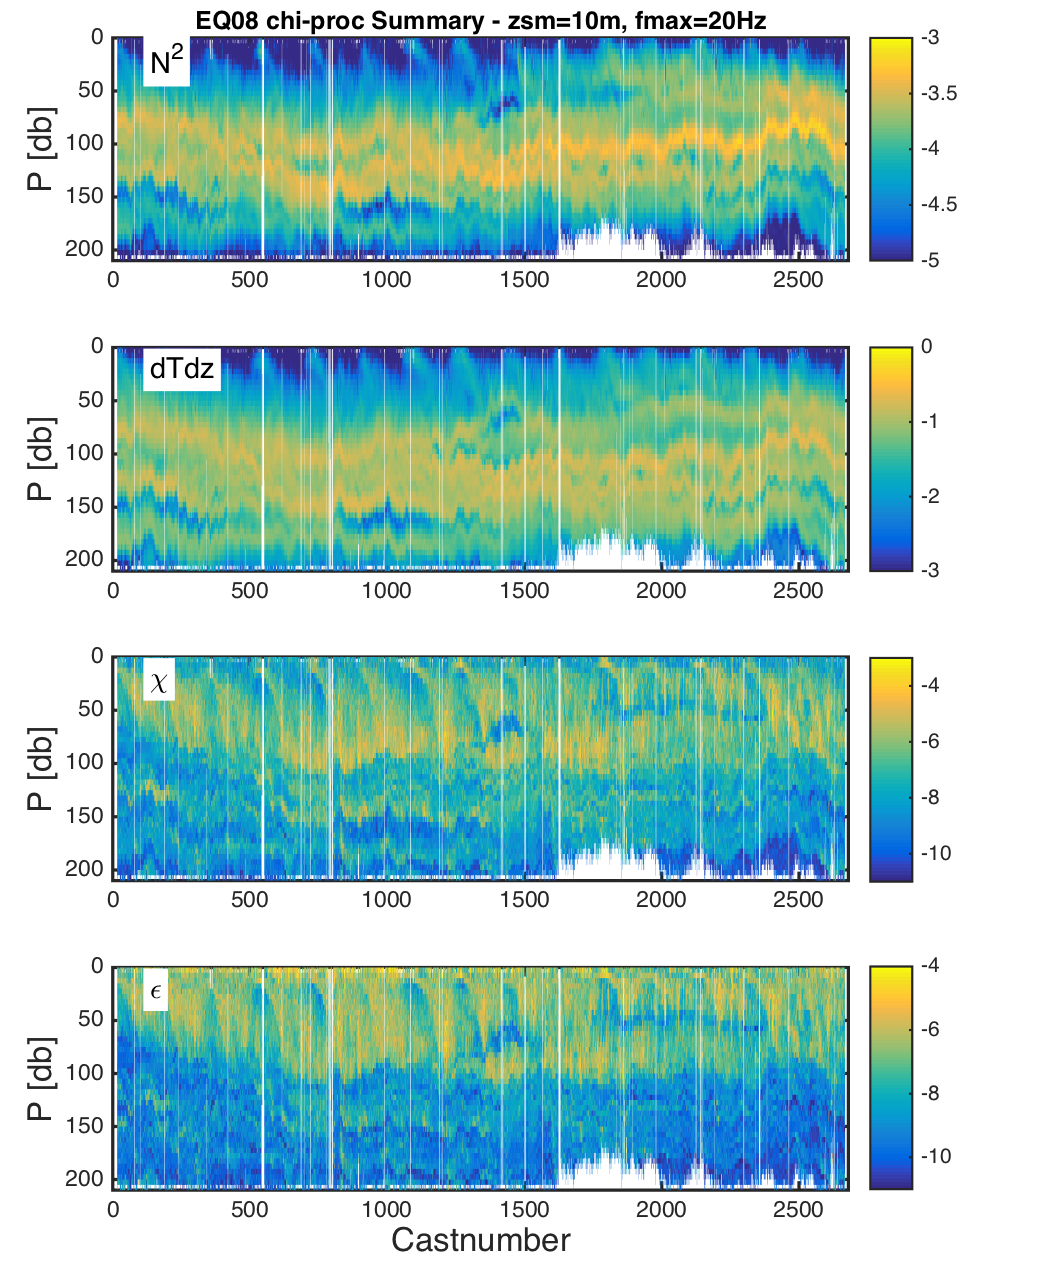
\includegraphics[scale=0.95]{EQ08_chiproc_Summary.png}
\caption{Summary of $\chi$pod method applied to Chameleon data from EQ08.}
\label{chi_sum}
\end{figure}


\clearpage
\newpage
%~~~~~~~~~~~~~~~~~~~~~~~~~~~~~
\section{Effect of Smoothing N2 and dTdz}

I ran $\chi$pod processing with different values of \verb+z_smooth+, the vertical scale over which $N^2$ and $dT/dz$ are averaged. Figure \ref{hist_dzsm} shows the results. $\chi$ is not affected very much, while $\epsilon$ tends to be increased for smaller values of zsmooth.


\begin{figure}[htbp]
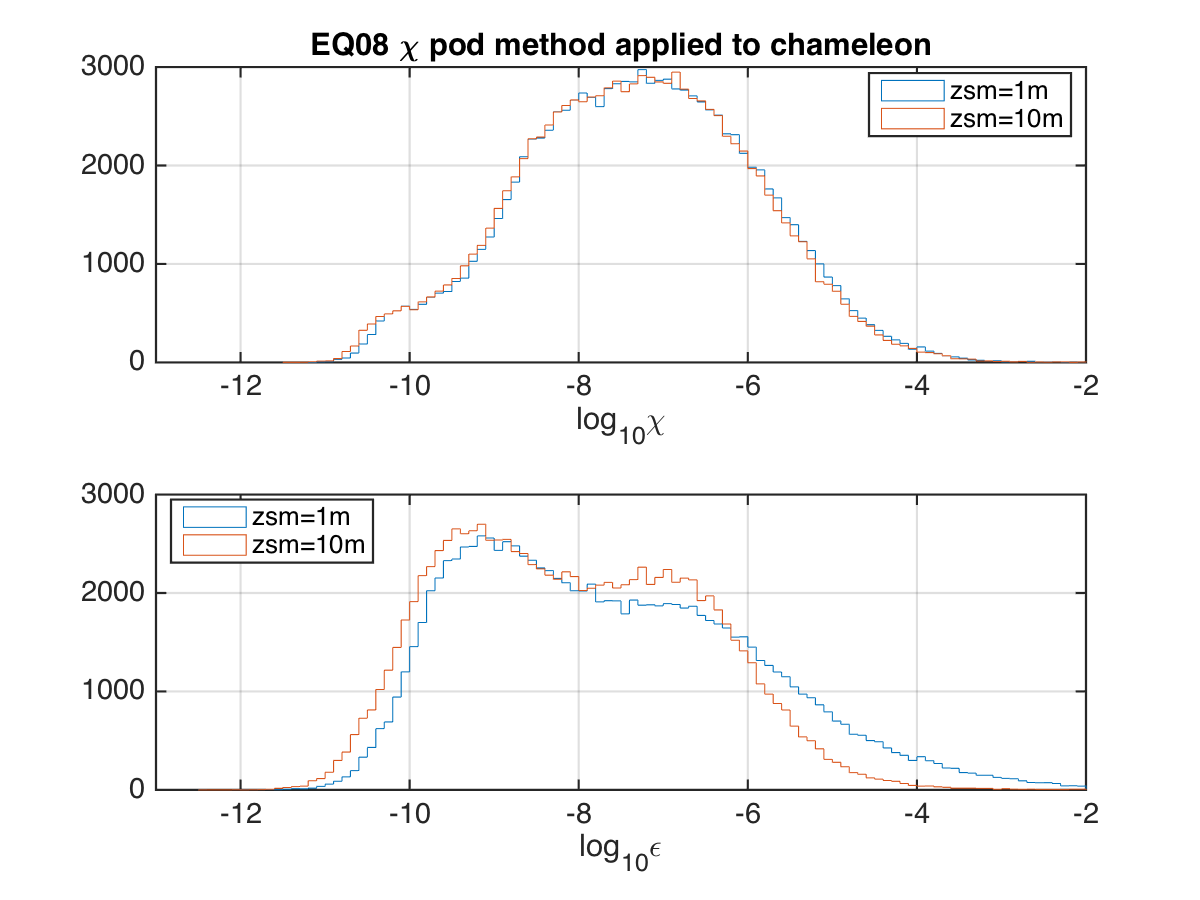
\includegraphics[scale=0.7]{hist_chi_eps_diff_zsmooth.png}
\caption{Histogram of $\chi$ and $\epsilon$ from $\chi$pod method and `true' chameleon data, for 2 different values of the `zsmooth' parameter.}
\label{hist_dzsm}
\end{figure}






\clearpage
\newpage
%~~~~~~~~~~~~~~~~~~~~~~~~~~~~~
\section{Effect of Frequency Response Correction}

Applying a frequency response correction to the dT/dt data does not appear to have much of an effect on the results (Figure \ref{hist_dresp}).

\begin{figure}[htbp]
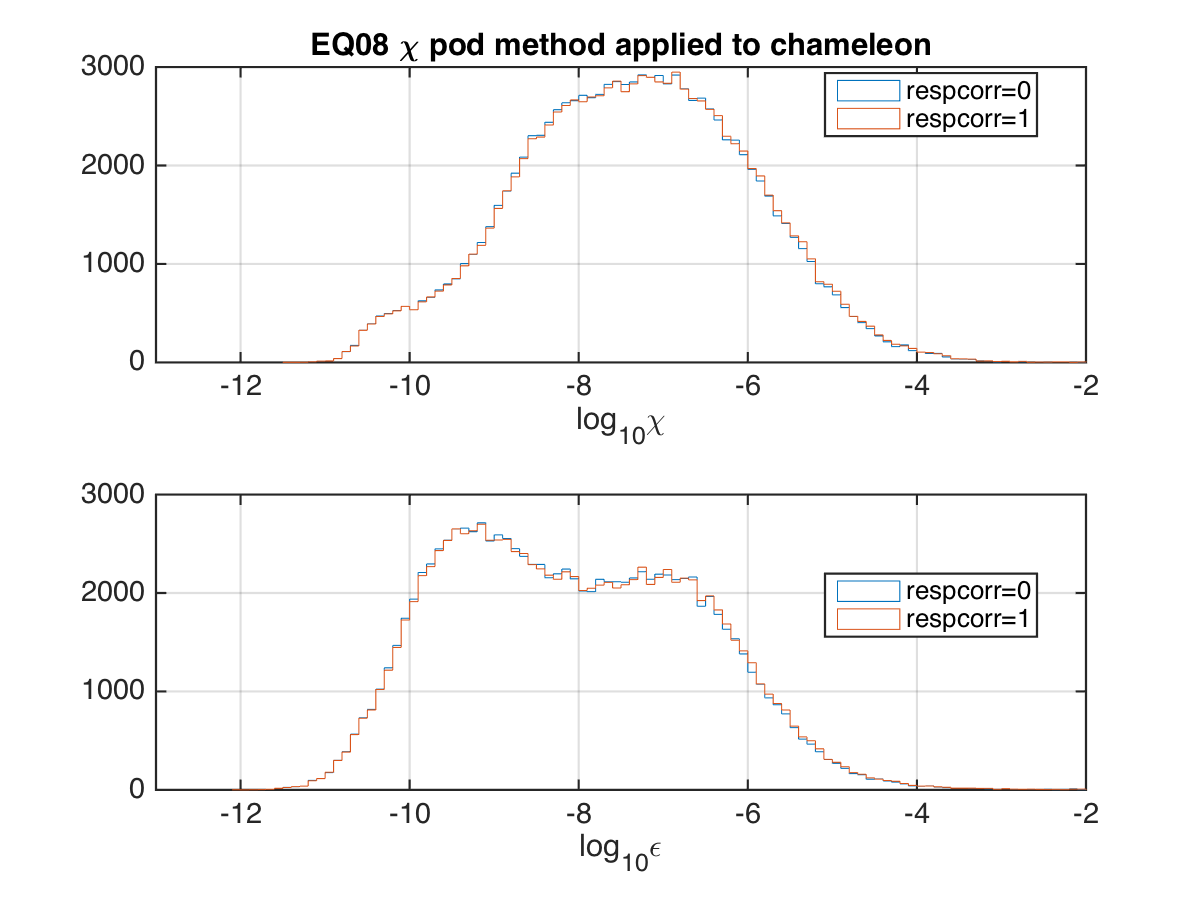
\includegraphics[scale=0.7]{hist_chi_eps_diff_respcorr.png}
\caption{Histogram of $\chi$ and $\epsilon$ from $\chi$pod method and `true' chameleon data, with and without frequency response correction.}
\label{hist_dresp}
\end{figure}






\clearpage
\newpage
%~~~~~~~~~~~~~~~~~~~~~~~~~~~~~
\section{Effect of `fmax' Parameter}

The `fmax' parameter sets the maximum frequency to integegrate the temperature gradient spectrum up to in \verb+get_chipod_chi.m+.

%\verb+Compare_chi_diff_fmax_EQ08.m+

\begin{figure}[htbp]
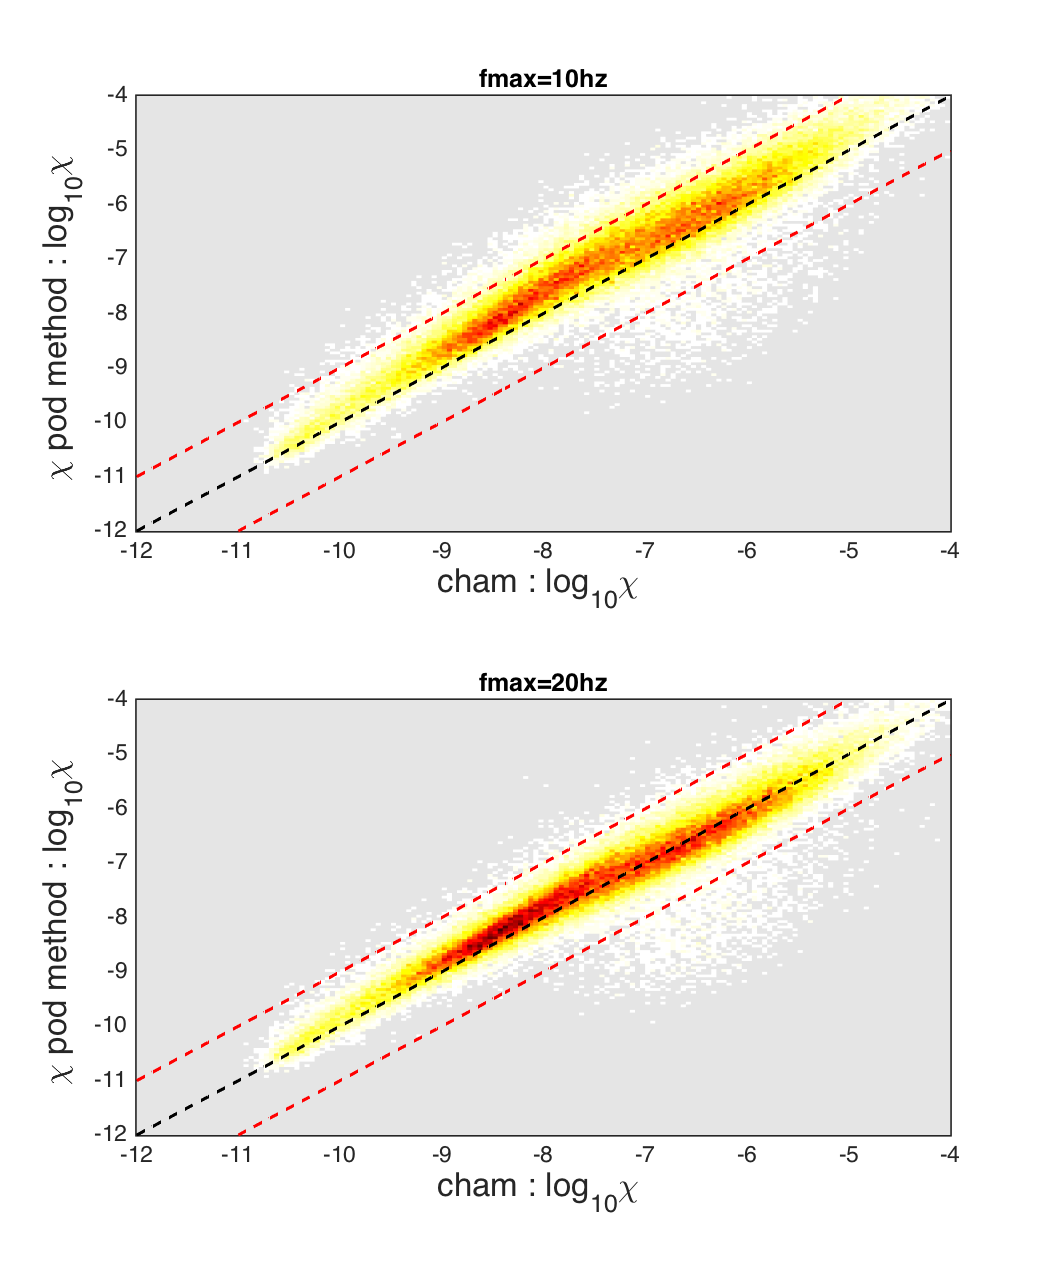
\includegraphics[scale=0.7]{2Dhist_chi_10mzsmooth_diff_fmax.png}
\caption{2D histogram of $\chi$ from $\chi$pod method and `true' chameleon data, for 2 different values of the `fmax' parameter. Black dashed line is 1:1, red is $\pm$ an order of magnitude.}
\label{}
\end{figure}

\begin{figure}[htbp]
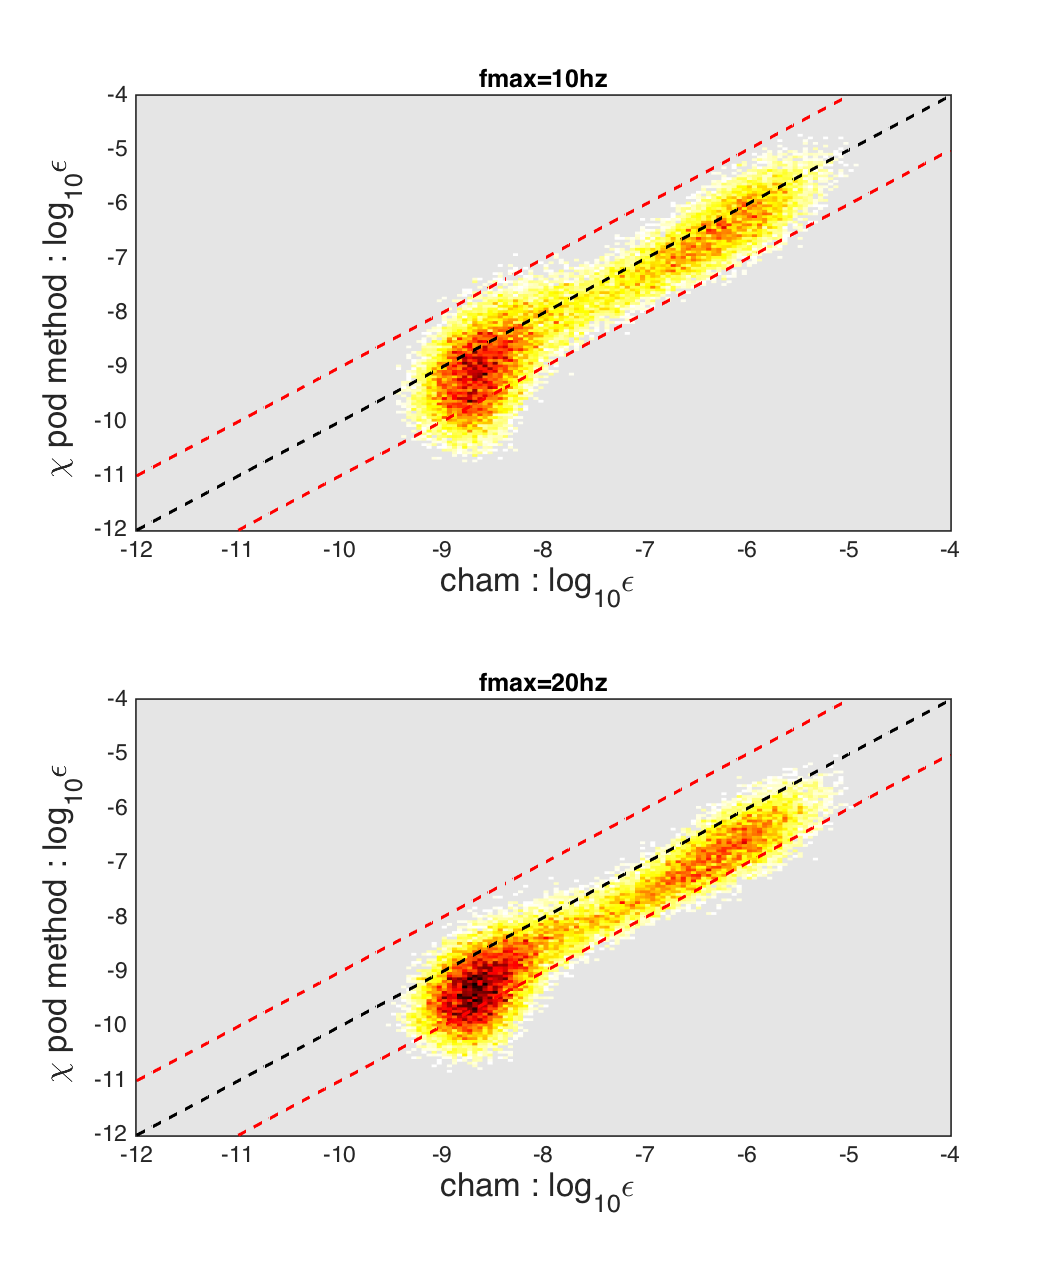
\includegraphics[scale=0.7]{2Dhist_eps_10mzsmooth_diff_fmax.png}
\caption{2D histogram of $\epsilon$ from $\chi$pod method and `true' chameleon data, for 2 different values of the `fmax' parameter. Black dashed line is 1:1, red is $\pm$ an order of magnitude.}
\label{}
\end{figure}




\clearpage
\newpage
%~~~~~~~~~~~~~~~~~~~~~~~~~~~~~
\section{$K_T$ versus $K_{\rho}$ in this dataset}

One of the assumptions made in the chipod method is that $K_T=K_{\rho}$. I tested this by computing these values in \verb+CompareKtKrho.m+ from chameleon data according to the formulas
\begin{eqnarray}
K_T=\frac{1}{2}\frac{\chi}{<dT/dz>^2} \\
K_{\rho}=0.2 \epsilon /N^2
\end{eqnarray}
where I use a mixing efficiency of $\Gamma=0.2$. It appears that $K_T$ is consistently smaller than $K_{\rho}$, by about a factor of 3-4 (Figure \ref{2dhist_Kt_Krho}).

\begin{figure}[htbp]
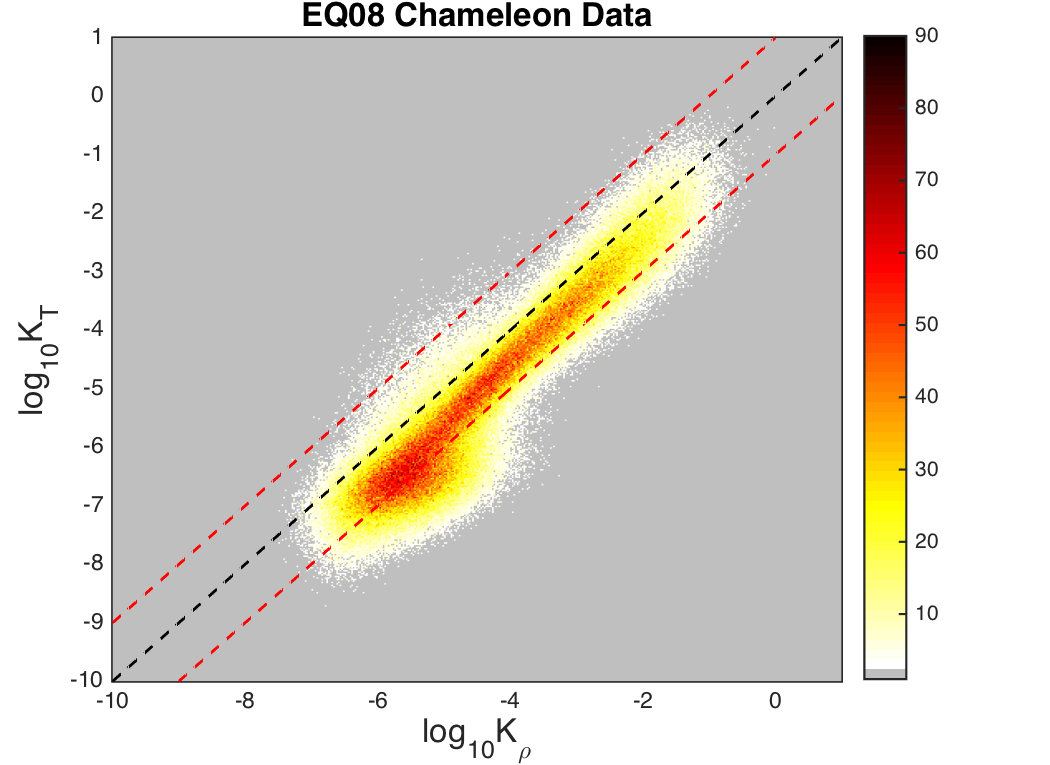
\includegraphics[scale=0.7]{Cham_KtVsKrho_2Dhist.png}
\caption{2D histogram of $K_T$ vs $K_{\rho}$ from chameleon data in EQ08. Black dashed line is 1:1, red is $\pm$ an order of magnitude.}
\label{2dhist_Kt_Krho}
\end{figure}


\begin{figure}[htbp]
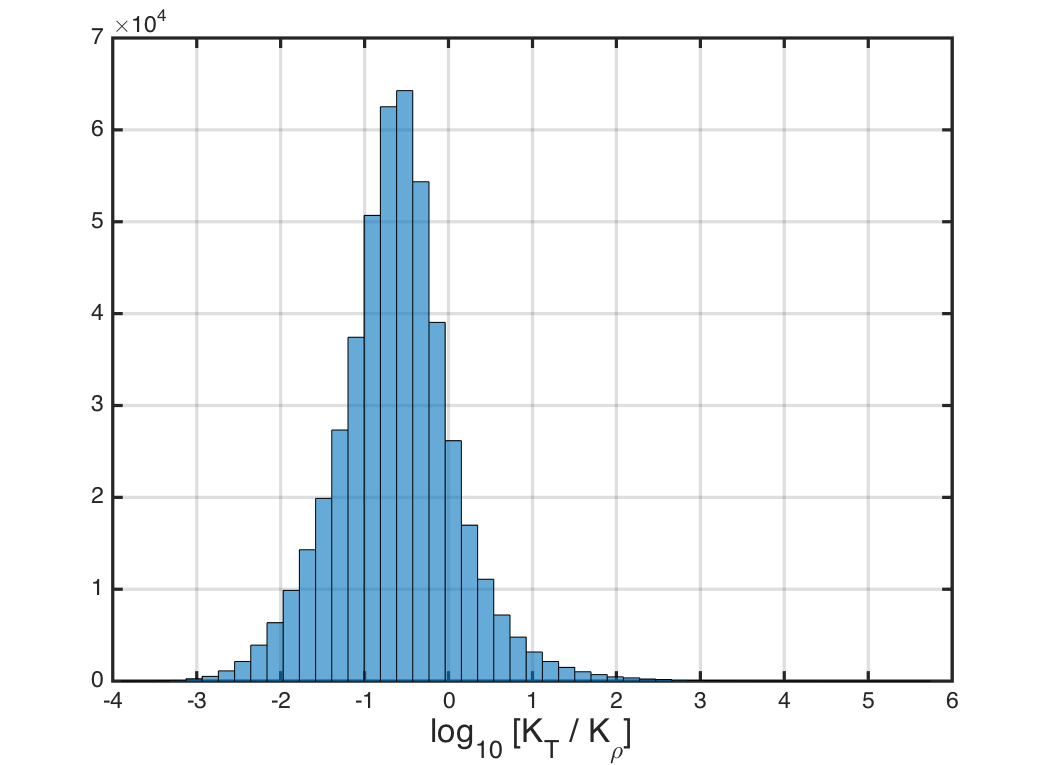
\includegraphics[scale=0.7]{Cham_Kt_Krho_hist.png}
\caption{Histogram of the ratio of $K_T$ to $K_{\rho}$ from chameleon data in EQ08.}
\label{}
\end{figure}





\clearpage
\newpage
%~~~~~~~~~~~~~~~~~~~~~~~~~~~~~
\section{Summary}

\begin{itemize}
\item Applying a frequency response correction has little/no effect.
\item Smaller values of zsmooth give similar $\chi$ but tend to produce larger $\epsilon$ values.
\item fmax affects the results; a value of 20Hz seems to give better agreement in $\chi$, but $\epsilon$ is smaller than the true values.
\item From chameleon data, $K_T$ is consistently less than $K_{\rho}$ by about a factor of 3-4. This could explain why the $\chi$pod $\epsilon$ values are smaller than the true values.
\end{itemize}



%~~~~~~~~~~~~~~~~~~~~~~~~~
 \bibliographystyle{ametsoc2014}
\bibliography{/Users/Andy/Cruises_Research/wavechasers_bib/main}





\end{document}  
